 % ****** Start of file apssamp.tex ******
%
%   This file is part of the APS files in the REVTeX 4.2 distribution.
%   Version 4.2a of REVTeX, December 2014
%
%   Copyright (c) 2014 The American Physical Society.
%
%   See the REVTeX 4 README file for restrictions and more information.
%
% TeX'ing this file requires that you have AMS-LaTeX 2.0 installed
% as well as the rest of the prerequisites for REVTeX 4.2
%
% See the REVTeX 4 README file
% It also requires running BibTeX. The commands are as follows:
%
%  1)  latex apssamp.tex
%  2)  bibtex apssamp
%  3)  latex apssamp.tex
%  4)  latex apssamp.tex
%
\documentclass[%
 reprint,
%superscriptaddress,
%groupedaddress,
%unsortedaddress,
%runinaddress,
%frontmatterverbose, 
%preprint,
%preprintnumbers,
%nofootinbib,
%nobibnotes,
%bibnotes,
 amsmath,amssymb,
 aps,prl,
%pra,
%prb,
%rmp,
%prstab,
%prstper,
floatfix
]{revtex4-2}

\usepackage{amsmath}
\usepackage{mathtools}
\usepackage{xcolor}
%\usepackage{caption}
%\usepackage{subcaption}
\usepackage{graphicx}% Include figure files
\usepackage{dcolumn}% Align table columns on decimal point
\usepackage{bm}% bold math
\usepackage{float}


%\usepackage{hyperref}% add hypertext capabilities
%\usepackage[mathlines]{lineno}% Enable numbering of text and display math
%\linenumbers\relax % Commence numbering lines

%\usepackage[showframe,%Uncomment any one of the following lines to test 
%%scale=0.7, marginratio={1:1, 2:3}, ignoreall,% default settings
%%text={7in,10in},centering,
%%margin=1.5in,
%%total={6.5in,8.75in}, top=1.2in, left=0.9in, includefoot,
%%height=10in,a5paper,hmargin={3cm,0.8in},
%]{geometry}
\newcommand{\Comment}[1]{\textcolor{red}{[#1]}}
\bibliographystyle{apsrev4-2}

\begin{document}
\preprint{APS/123-QED}
\title{Going Beyond the Cumulant Approximation:\\Power Series Correction to Single Particle Green's Function in Holstein System }
\author{Bipul Pandey}
\email{bipulpandey2004@uchicago.edu}
\author{Peter B. Littlewood}
\affiliation{Department of Physics, University of Chicago,Chicago, Illinois, 60637, USA}

\date{\today}% It is always \today, today,
             %  but any date may be explicitly specified

\begin{abstract}
In the context of a single electron two orbital Holstein system coupled to dispersionless bosons, we develop a general method to correct single particle Green’s function using a power series correction (PSC) scheme. We then outline the derivations of various flavors of cumulant approximation through the PSC scheme and explain the assumptions and approximations behind them. Finally, we compute and compare PSC spectral function with cumulant and exact diagonalized spectral functions and elucidate three regimes of this problem - two that cumulant explains and one where cumulant fails. We find that the exact and the PSC spectral functions match within spectral broadening across all three regimes.
\end{abstract}

%\keywords{Suggested keywords}%Use showkeys class option if keyword
                              %display desired
\maketitle

%\tableofcontents

\section{I. Overview:\protect}
Electrons and holes in materials undergo numerous complex interactions among themselves, the external fields, as well as the constituent atomic lattice. The strength of such many body interactions depends on various factors such as electronic configuration of the host material, presence of doping and defects, lattice parameters etc. Such factors manifest as bosonic collective excitations that renormalize the particle states (electrons/holes) into quasiparticles states with different energy and lifetime, and even mix quasiparticle states depending on the interaction strength. Alongside the quasiparticle features in photo-emission spectra, these collective excitations show up as "shake-off" features that can be loosely separated into sharp satellites emerging from bosonic collective modes (such as plasmons and optical phonons) and continua arising from non-zero-momentum particle-hole excitations (including excitons) \cite{goulielmakis_real-time_2010,lemell_real-time_2015,neppl_direct_2015}.

In calculations, the interaction strengths between collective excitations and particles are modeled as tunable electron-boson coupling parameters. In experiments, this coupling tunability is achieved by introducing doping and defects \cite{wang_tailoring_2016, kang_holstein_2018}. Although at very weak coupling the quasiparticle renormalization due to the collective modes is negligible, with stronger coupling a proportional renormalization of the quasiparticle occurs. As an example, in photo-emission spectra of strontium titanate this coupling manifests as a significant shift in quasiparticle energy, significant decrease in lifetime and intensity of quasiparticle features, strong shake-off features, as well as a strong mass enhancement of the carrier \cite{van_mechelen_electron-phonon_2008, devreese_many-body_2010, wang2016, swartz2018, edelman2021}. Strong electron-phonon coupling is also visible in electronic spectra in metallic cuprates \cite{rosch_polaronic_2005,damascelli_angle-resolved_2003} and the metal-insulator transition in undoped cuprates \cite{baldini_electronphonon-driven_2020}, and other correlated metals for example $FeSe/SrTiO_3$ epitaxial layers \cite{yang2015}.
At extreme values of coupling constant, strong electron-boson coupling can completely self-trap and localize electrons creating polaronic states. This severely alter carrier mobility in the material. This is of particular interest in the material design for photovoltaics and electronics \cite{mohamed_electronic_2019, ma_energy_2016, hulea_tunable_2006}. Finally, in the presence of multiple boson species, there can be competition between their effect on the carrier which creates novel phase crossovers in materials \cite{riley_crossover_2018}. Therefore a proper understanding and quantification of the effects of collective modes on charge carriers is vital in understanding and designing novel material with interesting engineering applications.

 In this work, we build on, and generalize, existing non-perturbative methods including the "GW" approximation \cite{hedin_new_1965} and the cumulant expansion \cite{langreth_singularities_1970} to describe the single particle dynamics of a system with multiple electronic levels interacting through common boson baths. The paper is organized as follows. In Section II, we introduce the model problem and the concepts of electron Green's function, electron self energy and cumulant corrections. In III, we briefly introduce the existing methods and their major drawbacks. In IV, we develop our correction scheme, and physically motivate the assumptions used to simplify the equations. In sections V, we outline the derivation of various flavors of cumulants through our method and elucidate the implicitly made but vaguely understood assumptions behind these approximation. Finally, in section VI, we identify three important regimes of the problem by comparing the performance of the cumulant method and the power series method with results from exact diagonalization of this problem in finite boson basis.
 %%%%%%%%%%%%%%%%%%%%%%%%%%%%%%%%%%%%%%%%%%%%%%%%%%%
\section{II. Introduction to the Problem}
 We consider a model Hamiltonian for a single electron two orbital Holstein system with bonding/anti-bonding energy $\varepsilon_+/\varepsilon_-$ such that their difference is $\Delta$. This system is kept in baths of two dispersionless boson species $(\pm)$. The bosons are quantized packets of energy $\omega_o$ that the electron can interact with. Interaction of electron with $(-)$ bosons causes an electron's inter-orbital transition. The $(+)$ boson does not cause any electronic transition upon interaction. 
 
 The electron-boson interaction strength is controlled by a coupling constant $g$. The fermionic ladder operators are $c_+/c_+^\dagger$ and $c_-/c_-^\dagger$ for bonding and anti-bonding orbitals respectively. The bosonic ladder operators for $(\pm$) bosons are $b_\pm /b_\pm^\dagger$. The Hamiltonian for this problem is separable into three distinct pieces. $H_o$ is the non-interacting part of the Hamiltonian. $H_+$ explicitly has $(+)$ bosons and doesn't cause inter-orbital transitions while $H_-$ explicitly has $(-)$ bosons and governs inter-orbital transitions.
\begin{equation}
\begin{aligned}
H\, &= H_o + H_+ + H_- \quad\text{where,} \\
H_o &= \sum_{i=\pm} \varepsilon_\pm c_i^\dagger c_i  \\
H_+ &=  \omega_o b_+^\dagger b_+ +  g(c_+^\dagger c_+ + c_-^\dagger c_-)(b_+^\dagger + b_+) \\
H_- &=  \omega_o b_-^\dagger b_- +g(c_+^\dagger c_- + c_-^\dagger c_+)(b_-^\dagger + b_-)
\end{aligned}
\label {Holstein}
\end{equation}
%%%%%%%%%%%%%%%%%%%%%%%%%%%
%%%%%%%%%%%%%%%%%%%%%%%%%
 Here $g$ is same in both $H_\pm$ due to the original problem's symmetries. But, even if they are different i.e $g_\pm$ in $H_\pm$, we can find corrections in powers of a dummy variable $g$ that multiplies both $g_\pm$ and set it to $1$ in the end.

This Hamiltonian describes the physics of a model of the dihydrogen cation $(H_2^+)$ - two hydrogen nuclei and a single electron. Historically, this problem was approached with clamped nuclei approximation. This crude approach completely neglects the vibronic coupling between the electron and vibrational modes of the nuclei (optical phonons in crystalline structures - see supplement) which becomes crucial when $\Delta \approx \omega_o$. Vibronic couplings in this regime can cause inter-band transitions and severely renormalize the energy levels in the molecule \cite{heller_molecular_1979,heller_molecular_1980, ranninger_two-site_1992}. Hence, this is a good model to construct the approximation scheme due of its simplicity and similarities to real multi-level systems. Furthermore, no exact analytical solution exists and the approximate methods either give incorrect boson satellites (GW) or are {\it ad hoc}, unsystematic and incorrect at strong coupling (cumulant) \cite{gunnarsson_corrections_1994}. 
%%%%%%%%%%%%%%%%%%%%%%%%%%%%%%%%%%%%%%%%
%%%%%%%%%%%%%%%%%%%%%%%%%%%%%%%%%%%%%%%%%

%\subsection{Electron Green's Function and Spectral Function}
\textbf{The Green's function:}
The retarded-time(RT) formalism is better suited to handle electron-hole interactions because it treats both of them in equal footing as particles \cite{kas_cumulant_2014}. For the Holstein problem \eqref{Holstein} with fock vacuum $|0\rangle$ as the ground state and \{ , \}/[ , ] as the anti-commutator/commutator, The electron Green's function $G(n,t)$ for each orbital ($n=\pm$) and the boson Green's function $\mathcal{D}(N,t)$ for each boson species $(N =\pm)$ in retarded formalism is given by;
\begin{equation}
\begin{aligned}
    G(n,t) &= -i \theta(t)\langle 0|\{c_n(t) ,{c_n^{\dagger}}\}|0\rangle\\
    \mathcal{D}(N,t) &= -i \theta(t)\langle 0|[b_N(t) ,{b_N^{\dagger}}]|0\rangle\\
\end{aligned}
\label{Greens definition}
\end{equation}
For non-interacting(g=0) electrons and dispersionless bosons with energy $\omega_o$, the bare electron green's function $G_o$ and a bare boson green's function $\mathcal{D}$ are,
\begin{equation}
\begin{aligned}
G_o(\pm,t) = -i\theta(t) e^{-i\varepsilon_\pm t} \\ \mathcal{D}(\pm,t) = -i\theta(t)e^{-i\omega_o t}
\end{aligned}
\label{Bare electron and boson greens and greens}
\end{equation}

The quasiparticle energies, lifetimes and the boson satellites show up as complex poles of $G(n,\omega)$ where $\omega$ is the frequency. The frequency axis spectral function, $A(m,n;\omega)$ (see supplement) is defined as;
 \begin{equation}
     A(m,n;\omega) = \frac{1}{\pi} |\text{Im}G(m,n;\omega)|
 \end{equation}
%%%%%%%%%%%%%%%%%%%%%%%%%%%%%%%%%%%%%%%%%
%\subsection{Electron Self Energy and Dyson's equation}
\textbf{Electron self energy and Dyson's equation: }
  At zero coupling ($g=0$), the energy eigenvalues $\varepsilon_{\pm}$ of \eqref{Holstein} are real and the states have infinite lifetime owing to the lack of interaction between the orbitals. However, upon switching on the boson mediated interaction ($g\neq0$) between orbitals, the exchange of energy and momenta between states through boson exchange causes clumping of electrons and holes to form quasiparticles. Because of time-transnational invariance, we can package this interaction information together and call it the self energy.
\begin{equation}
    -i\Sigma(t) = g^2\!\sum_{\substack{N=\pm\\n=\pm}} \mathcal{D}(N,t)G(n, t)= g^2 \!\sum_{n = \pm}\!\!\!-i\Sigma(n,t)
\label{self-energy}
\end{equation}
Each orbital's self energy $\Sigma(n, t)$ is complex valued unlike the bare energy. This gives rise to spectral peak broadening - an indicative of finite quasiparticle lifetime. A properly constructed self energy also incorporates boson mediated inter-orbital transitions, produces satellite peaks at the correct boson frequencies and redistributes the spectral weight from the quasiparticle to the satellites. The Dyson's equation governs the evolution of electron Green's function by repeated application of this self energy.
\begin{equation}
  G(n,\omega) = G_o(n,\omega) + G_o(n,\omega)\Sigma(\omega) G(n,\omega)
  \label{Dyson equation}
\end{equation}
%%%%%%%%%%%%%%%%%%%%%%%%%%%%%%%%%%%%%%%%%
\section{III. GW, Cumulant Expansion and Their Drawbacks}
The $GW$ approximation used to compute the quasiparticle properties are non self consistent and have abrupt truncation of Dyson's equation for computational efficiency unlike the fully self-consistent original $GW\Gamma$ formalism \cite{hedin_new_1965}. Although $GW$ based methods give reasonably good description of quasiparticle properties at weak coupling, the plasmon satellites are averaged and misplaced at some incorrect average energy \cite{langreth_singularities_1970}. At strong coupling, due to the lack of self-consistency, even the quasiparticle properties can be incorrect.

For a single (or isolated) band of electrons in a dispersionless plasmon bath \cite{langreth_singularities_1970}, an exact solution of the following form exists.
\begin{equation}
G(k,t) = G_o(k,t) e^{C(k,t)}
\label{cumulant}
\end{equation} 
The cumulant $C(k,t)$ is calculated by comparing equation \eqref{cumulant}'s taylor-expansion with the temporal Dyson's equation with $G$ and $\Sigma$ obtained from GW \cite{aryasetiawan_multiple_1996}. The satellites manifest as a Poisson series of peaks plasma frequency apart in the spectral function due to the exponential form of the cumulant ansatz \eqref{cumulant}. In real systems, although not all assumptions of above model hold true, an approximate cumulant correction can be found using the same recipe as above on a GW self energy. Recently, interest in the cumulant approximation has re-surged \cite{kas_cumulant_2014,gumhalter_combined_2016,caruso_band_2015,lischner_physical_2013} enabled by increases in computational ability to perform $GW$ and inspired by experiments (.e.g. \cite{guzzo_multiple_2014}) on complex systems.

The cumulant has the considerable merit of giving near-exact spectra for weak electron-boson coupling- $\Delta\gg\omega_o$ and/or $g\ll1$. However, at strong coupling and presence of multiple electronic levels, the bosons significantly affect the quasi-particle properties in ways not reflected in the cumulant approximation. The cumulant is also not systematically improvable by design and lacks proper accounting of inter-band scattering owing to the absence of self-consistency. 

\section{IV.Theoretical Framework:}
%\subsection{ Power Series Ansatz and its Properties %\protect}
\textbf{The Power Series Ansatz: }Rather than assuming an exponential correction, we assume a power series correction $\mathcal{P}(n,t)$ in the powers of  $g^2$ to the $n^{th}$ orbital's electron bare Green's function $G_o(n,t)$ due to interaction with bosons for time duration `t'. By construction, the interacting system smoothly maps to the non interacting system as $g^2$ goes to zero. 
\begin{equation}
\begin{aligned}
    G(n,t) = G_o(n,t) \mathcal{P}(n,t) = G_o(n,t)\sum_{k=0}^\infty g^{2k} C_k(n,t)
\end{aligned}
\label{eq:Corrected_Greens}
\end{equation}
Here $C_0 = 1$ and all other $C_k$ are distinct correction functions of different orders that are 0 when $t<0$. This makes physical sense because in retarded time framework- the particle doesn't exist for $t<0$. This, just like cumulant, is still a diagonal approximation to the Green's function matrix because, by construction, only those corrections in which a particle eventually returns back to its initial state $n$ are accounted for. 

\textbf{Temporal contraction relation: } For a given orbital n and time $t_i<t_o<t_f$, both $G$ and $G_o$ and hence by inheritance $\mathcal{P}$ have the following temporal contraction property due to the boundary value dependence on time. 
\begin{equation}
    f(n,t_f-t_i) = f(n,t_f-t_o)f(n,t_o-t_i)
    \label{contraction}
\end{equation}
This property doesn't apply between these function for different orbitals. In calculations, this seemingly trivial property of $\mathcal{P}(n,t)$ is absolutely essential to account for bosonic crossing diagrams. 

%%%%%%%%%%%%%%%%%%%%%%%%%%%%%%%%%%%%%%%%%%%%%%%%%%%%%%%%%%%%%%%%%%%%%%%%
%\subsection{Assumption on Electron Self Energy}
\textbf{Assumption on Electron Self Energy: }To properly construct the electron self energy, rather than replacing $G$ by $G_o$ inside the self energy as in $GW$ or cumulant expansions, we replace it by power series ansatz in order to re-introduce self-consistency.
%%%%%%%%%%%%%%%%%%%%%%%%%
%%%%%%%%%%%%%%%%%%%%%%%%%
\begin{equation}
\begin{aligned}
    -i\Sigma(t) &= g^2 \sum_{n=\pm}\,\sum_{N= \pm} \mathcal{D}(N,t)G_o(n, t)\mathcal{P}(n,t)\\
    &=g^2 \sum_{n=\pm}-i\Sigma_o(n,t)\mathcal{P}(n,t)
\end{aligned}
\label{Power corrected self energy}
\end{equation}
Here, the $n^{th}$ orbital's self-energy $\Sigma_o(n,t)$ computed by using bare Green's function $G_o$. The introduction of power series in $\Sigma$ through $G$ now produces corrections due to the particle's eventual return to the initial state after scattering through other possible states. Including these cyclic scattering contributions in the Green's function matrix's diagonal makes the diagonal exact.

%%%%%%%%%%%%%%%%%%%%%%%%%%%%%%%%%%%%%%%%%%%%%%%%%%%%%%%%%%%%%%%%%%%%%%%%%%%%%%%%%
%\subsection{Correction Scheme}
\textbf{Correction Scheme: }We take the temporal Dyson's equation for $m^{th}$ band and replace $G$ and $\Sigma$ by their power series corrected versions from \eqref{eq:Corrected_Greens}, \eqref{Power corrected self energy}. We then use the temporal limits enforced by the RT bare Green's function \eqref{Bare electron and boson greens and  greens} and simplify the equation using the temporal contraction property from equation \eqref{contraction}. 
 \begin{figure}
    \centering
    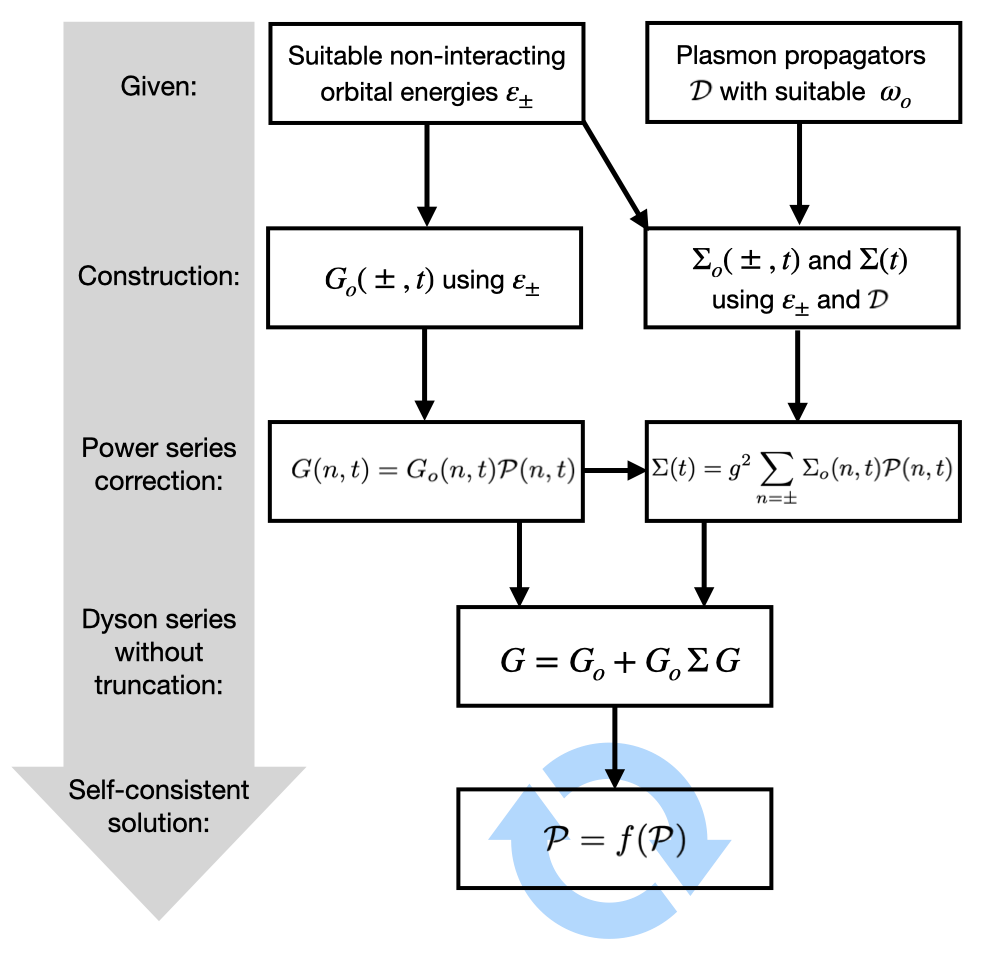
\includegraphics[height = 9 cm,width = 0.48\textwidth]{Flow_chart.001.png}
    \caption{Flow chart of the Correction Scheme}
    \label{Flow Chart}
\end{figure}
\begin{equation*}
\begin{split}
     G(m,t-t_0) &=  G_o(m,t-t_0) \quad +\\
     \!\!\iint d{t_1} &d{t_2} G_o(m,t-t_2)\Sigma(t_2-t_1)G(m,t_1-t_0)
\end{split}
\end{equation*}
Setting $t_0=0$ and $t_2-t_1 = \tau$, and simplifying, we get,
\begin{equation*}
\begin{split}
    \mathcal{P}(m,t) =  \quad 1 &\quad+\\
    (-ig^2)\sum_{n=\pm}\int\displaylimits_{0}^{t} & \! dt_2 \!\!\int \displaylimits_{0}^{t_2}\!\!d \tau  e^{i\varepsilon_{m}\tau}\Sigma_o(n,\tau)\mathcal{P}(n,\tau) \mathcal{P}(m,t_2-\tau)
\end{split}
\end{equation*}
There are two distinct terms in this equation. The self correction ($P_{SC}$) term occurs when the interaction is within same orbital ($n=m$) on the right side of this equation. Here, the contraction property \eqref{contraction} must be used between the power series pieces on the right. The inter-band scattering term ($P_{IC}$) occurs when different orbitals interact ($n\neq m$) and here the contraction property is no longer valid. 
\begin{equation}
    \begin{aligned}
    &\therefore \mathcal{P}(m,t) =  1 + P_{SC} + P_{IC}\quad \quad\text{where,}\\
    &P_{SC}=\! -ig^2\!\!\int\displaylimits_{0}^{t}\!\!dt_2 \!\int\displaylimits_{0}^{t_2}\!\!d{\tau}\, e^{i\varepsilon_{m}\tau}\Sigma_o(m,\tau)\mathcal{P}(m,t_2)\\
     &P_{IC}= -ig^2\!\!\int\displaylimits_{0}^{t}\!\!dt_2 \!\!\int\displaylimits_{0}^{t_2}\!\!d\tau\, e^{i\varepsilon_{m}\tau} \,\Sigma_o(n,\tau)\mathcal{P}(n,\tau)\mathcal{P}(m,t_2-\tau)\\
    \end{aligned}
    \label{Power_Corr_full}
\end{equation}
For numerical solution, we start with an initial guess of $\mathcal{P} = 1$ on the right and self consistently compute better values for $\mathcal{P}$ on the left until it converges. 
%%%%%%%%%%%%%%%%%%%%%%%%%%%%%%%%%%%%%%%%%%%%%%

\section{V. Derivation of Various Cumulant Schemes }
We validate our method by deriving the exact cumulant result for the core-hole problem with single orbital of bare energy $\varepsilon_o$ in a bath of dispersionless plasmons of frequency $\omega_o$ \cite{langreth_singularities_1970}. The Hamiltonian in this case is;
\begin{equation*}
    \label{Core hole}
    H = \varepsilon_o c^\dagger c + \omega_o b^\dagger b + g (b^\dagger + b)(c^\dagger c -1)
\end{equation*}
This is an idealization of an isolated electron energy level $\varepsilon_o$ deep under the Fermi level being probed using x-ray photo-emission \cite{offi_comparison_2007}. The energetic electron exiting the system leaves behind a hole and the electron cloud responds to this imbalance of Coulomb forces by undergoing quantized long range oscillations (plasmons) at multiples of $\omega_o$. The corrected self energy for this case is;
\begin{equation*}
        \Sigma(t) \,= g^2 \Sigma_o(t)\mathcal{P}(t)\, =\, g^2 \big[-ie^{-i(\varepsilon_o-\omega_o)t} \theta(t)\big] \mathcal{P}(t)
\end{equation*}
For a single energy level, there is no inter-band scattering correction in equation \eqref{Power_Corr_full}.
\begin{equation*}
    \begin{aligned}
        \mathcal{P}(t)=1+ \Big[-ig^2\!\!\int\displaylimits_{0}^{t} dt_2 \int\displaylimits_{0}^{t_2}\!\!d{\tau}\, e^{i\varepsilon_{o}\tau}\Sigma_o(\tau)\mathcal{P}(t_2)\Big]
    \end{aligned}
    \label{single-disp-boson}
\end{equation*}

Expanding power series on both sides and comparing terms of same order in $g^2$ across the equality, we generate the following higher order corrections.
\begin{equation*}
    C_1(t) = \Big[\frac{e^{i\omega_o t} - i\omega_o t -1}{\omega_o^2}\Big] \quad \text{and}\quad C_k (t) = \frac{C_1(t)^k}{k!}
\end{equation*}
Summing all of these corrections gives us the exact result for the core hole problem.
\begin{equation}
G(t) = G_o(t)\mathcal{P}(t) = G_o(t)e^{g^2 C_1(t)}
\label{core-hole-cumulant}
\end{equation}

 The time-ordered cumulant expression in \cite{aryasetiawan_multiple_1996,gumhalter_combined_2016, caruso_band_2015,lischner_physical_2013} was derived assuming that the $n^{th}$ orbital's cumulant $C(n,t)$ depends only on the $n^{th}$ orbital's self energy $\Sigma(n,t)$ - thereby neglecting boson mediated inter-band scattering effects. In power series language, this translates as neglecting the effect of $H_-$ by setting $P_{IC}$ to be 0. In Holstein model, this means that the band gap $\Delta \gg \omega_o$ and each orbital essentially is an independent core-hole problem with corrections governed by $P_{SC}$ alone.

In the other limit - $\Delta \ll \omega_o$, the satellites are so far away that they don't modify the quasiparticle appreciably. Hence, both $P_{SC}$  and $P_{IC}$ are small and scale roughly equally. So they can be approximated as being independent of the orbital index in \eqref{Power_Corr_full}. This orbital independence lets us use the temporal contraction \eqref{contraction} for $P_{IC}$ regardless of orbital identity thereby giving RT cumulant correction \cite{kas_cumulant_2014,guzzo_multiple_2014}. The details of both derivations can be found in the supplement to this paper.
%%%%%%%%%%%%%%%%%%%%%%%%%%%%%%%%%%%%%%%%%%%%%%
\section{VI. Comparison with Exact Diagonalization Result}
\begin{figure}[htp]
    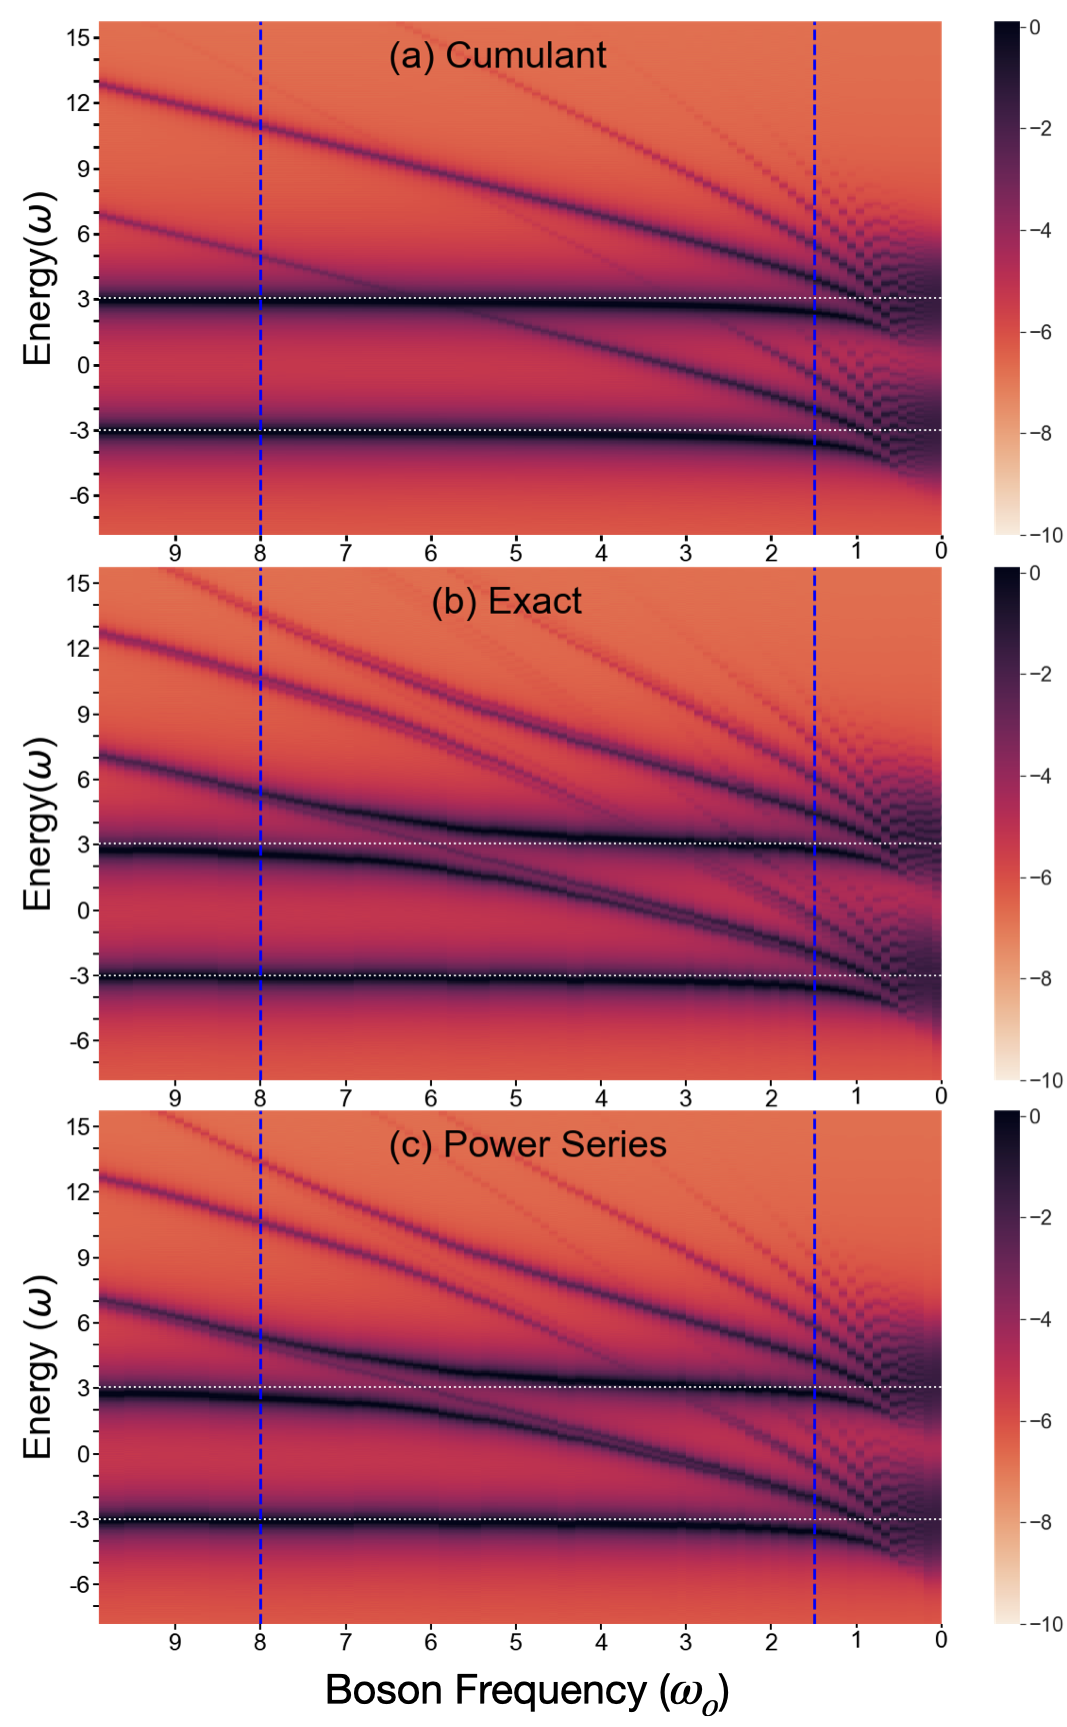
\includegraphics[height = 11.6 cm,width = 0.47\textwidth]{Final_Diagram_abs.png}
    \caption{Natural log of spectral function from a) RT cumulant, b) exact diagonalization, and c) power series for $\varepsilon_\pm = \mp3$ (horizontal white dotted lines) and $\omega_o$ between 10 and 0.1. The blue vertical lines separate the three distinct regions.}
    \label{three graphs}
\end{figure}
We now numerically compute and compare the spectral functions obtained from power series, the exact diagonalization ($N\geq40$ boson basis) and RT cumulant for problem \eqref{Holstein} with $\varepsilon_\mp = \pm 3$, $\omega_o$ from 10 to 0.1, spectral broadening of 0.1, and a strong coupling parameter of $g=1$ in figure \ref{three graphs}. Depending on the magnitude of $\omega_o$ with respect to $\Delta$, figure \ref{three graphs} separates into three distinct regions roughly demarcated by the dashed blue lines.

 The first region is the weak coupling regime of $\omega_o\! \gg\! \Delta$ - here $\omega_o\!>\!8$. Here, both $(\pm)$ plasmon satellites are far away from the quasiparticle and therefore their effect on the quasiparticle energy and weight is negligible. This is most prominently seen from the negligible change quasiparticle energy from the non-interacting energies $\varepsilon_\pm$. Here, the retarded cumulant adequately captures all the exact spectral features correctly.
\begin{figure}[htp]
    \centering
    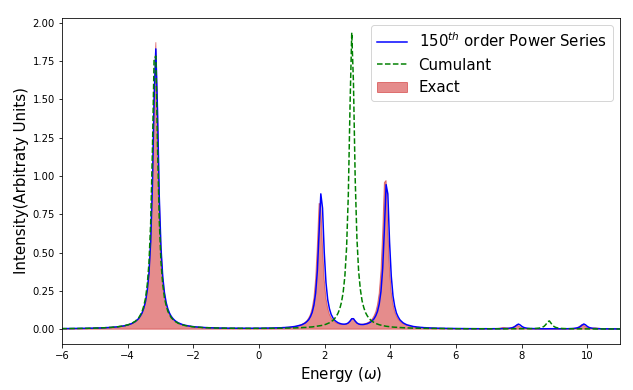
\includegraphics[height = 4.5 cm, width = 0.45\textwidth]{Spectra_at_boson_freq_6_emis.png}
    \caption{Spectral function with $g=1$, $\varepsilon_\pm = \mp3$, and $\omega_o =6$ from the three methods. Power series, unlike cumulant, captures the anti-bonding orbital splitting.}
    \label{omega_equals_delta}
\end{figure}

The second region has $\omega_o \approx \Delta$ - here $8>\omega_o>1.5$. A huge shift of spectral weight occurs from bonding to the anti-bonding orbital effectively splitting the anti-bonding orbital into two (between $\omega_o$ of 4 and 7). The shake-off replicas of this split level also come in pairs as seen in the exact spectra in figure \ref{omega_equals_delta}. These are captured exactly by the power series but not by cumulant because it lacks proper accounting of inter-band interaction.

The third region is when $\omega_o \ll \Delta$ - here $\omega_o < 1.5$. Here the bosonic events are extremely localized around the non-interacting energy and (+) bosons dominate the process. Therefore, inter-band interaction is vanishingly small and the solution is dominated by self-correction i.e core-hole like cumulant. We observe this in all three spectral functions although both exact and power series solution become computationally expensive -  the former due to large boson number necessary and the latter due to small time-step and large convergence order.

%%%%%%%%%%%%%%%%%%%%%%%%%%%%%%%%%%%%%%%%%%%%%%
\section{VII. Conclusion}
In this work, we derived a general power series based method which mitigates all the problems of cumulant-based methods, is practical to implement and reproduces the exact result in a finite basis for this problem within the spectral broadening used. We also identified three important regimes of this problem and elucidated where cumulant works, why cumulant works, and when it fails. We hope to extend this work to real multi-electron systems with strong plasmon resonances. 
 
%\nocite{*}
\bibliography{Power_Series_5}% Produces the bibliography via BibTeX.

\end{document}
%
% ****** End of file apssamp.tex ******
